\documentclass[12pt,fleqn]{article}

\usepackage{fullpage}
\usepackage[round]{natbib}
\usepackage{multirow}
\usepackage{booktabs}
\usepackage{tabularx}
\usepackage{tcolorbox}
\usepackage{graphicx}
\usepackage{float}
\usepackage{hyperref}
\hypersetup{
    colorlinks,
    citecolor=black,
    filecolor=black,
    linkcolor=black,
    urlcolor=blue
}
\oddsidemargin 0mm
\evensidemargin 0mm
\textwidth 160mm
\textheight 200mm

\usepackage{fancyhdr}
\fancyhead[L]{November 26, 2017}
\fancyhead[C]{SE 3XA3: Requirements Specification}
\fancyhead[R]{AKT}
\renewcommand{\headrulewidth}{0.4pt}

\pagestyle{fancy}
\usepackage[margin=2.5cm,headsep=.2in ]{geometry}

\pagenumbering{arabic}

\newcounter{stepnum}

\title{Group 29 (AKT)\\ Requirements Specification}
\author{
Alex Trudeau\\
	\texttt{400030148}
\and
Kathryn Kodama\\
  	\texttt{400013582}
\and
Tommy Tran\\
	\texttt{001150067}
}
\date{\today\\Version 2.0}

% Image directory
\graphicspath{{img/}}

\begin{document}

\maketitle

\pagebreak
\tableofcontents
\listoftables
\listoffigures

\begin{table}[ht]
\caption{\bf Revision History}
\begin{tabularx}{\textwidth}{p{3cm}p{2cm}X}
\toprule {\bf Version} & {\bf Date} & {\bf Notes}\\
\midrule
1.0 & 04/10/17 & Created document \\
1.1 & 05/10/17 & Updated document \\
1.2 & 06/10/17 & Finalized document Rev. 0 \\
2.0 & 26/11/17 & Started Rev.1 \\
\bottomrule
\end{tabularx}
\end{table}

\clearpage
 


\section {Project Drivers}

\subsection {Purpose of the Project}
The purpose of the project is to create a community based social news aggregator and message board. Users are able to rate posts based on their interest. Posts are then sorted from highest to lowest rated, essentially allowing for more interesting topics to be shown to a greater audience. In addition to viewing posts, users will be able to comment and discuss within each post.  This will facilitate the creation of and discussion within online communities.

\subsection {Stakeholders}

There are multiple stakeholders for this application as listed below.

\subsubsection* {The Customer/End Users}
\begin{itemize} 
\item \textbf{Application Registered Users: }The primary customers of this project are the application registered users. These are members of the general public who have an authenticated profile within the application and post and update shared content.
\item \textbf{General Public: }The secondary customers of this project are the general public users who browse the content without contributing and curating content.
\end{itemize}
\subsubsection* {The Principals and Partners}
\begin{itemize}
    \item \textbf{AKT Team: } The AKT Team are the developers of this project.  The team is involved in the creation and maintenance of the project.  In this case, the developers are the principal stakeholders as well as the producers.
    \item \textbf{Google Firebase: } Other producer stakeholders including Google Firebase as they are hosting the application and providing user authentication and database services.
\end{itemize}


%%%%%%%%%%%%%%%%%%%%%%%%%%%%%%%%%%%%%%%%%%%%%%%%

\pagebreak

\section {Project Constraints}

\subsection {Mandated Constraints}
\subsubsection{Solution Constraints}
\begin{tcolorbox}
\textbf{Description:} The application shall operate on devices modern web browsers.
\\
\textbf{Rationale:} The users include anyone with a device that can operate a web browser.
\\
\textbf{Fit Criterion:} The application shall be tested to be functional on web browsers across several devices.
\end{tcolorbox}

\begin{tcolorbox}
\textbf{Description:} The application shall operate only when the device is connected to the internet.
\\
\textbf{Rationale:} In order to submit content or participate in discussions, users require an internet connection.
\\
\textbf{Fit Criterion:} The application shall not load content without an internet connection.
\end{tcolorbox}


\subsubsection {Implementation Environment of the Current System}
\begin{figure}[htp]
\centering
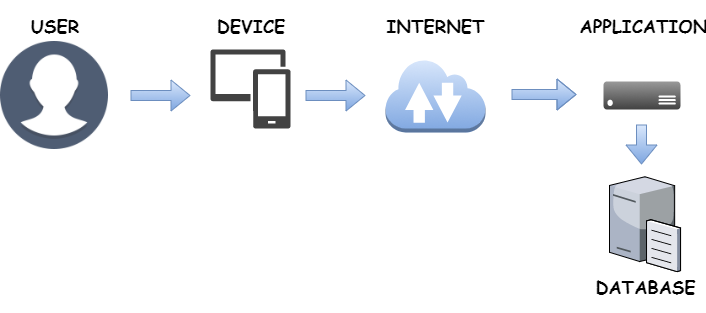
\includegraphics[width=16cm]{env}
\caption{Implementation Environment Diagram}
\label{fig:environment}
\end{figure}

\subsubsection {Partner or Collaborative Applications}
The application will leverage Google Firebase's services in order to handle user authentication, database communication and web server hosting.

\subsubsection {Off-the-Shelf Software}
The application requires that the user have a device that is able to connect to the internet and operate a web browser(Chrome, Firefox, Safari, Edge, Opera, etc). 

\subsubsection {Schedule Constraints}
The proof of concept demonstration application must be completed by October 16, 2017. \\
The application must be completed by December 6, 2017.  The development team can choose to maintain and update the project at their convenience after this date.

%%%%%%%%%%%%%%%%%%%%%%%%%%%%%%%%%%%%%%%%%%%%%%%%

\subsection {Naming Conventions and Terminology}

The naming conventions of this project have been agreed upon by the AKT development team.  Lower case Camel-Case will be closely followed when writing code.  Additionally, constants and enums will be identified with all capital naming conventions.  Each page and component of the code will follow standard ionic project naming conventions. For example, the homepage of the project will be named as follows: home.html, home.module.ts, home.scss, home.ts. 

\begin{table}[H]
\caption{\bf Terminology }
\begin{tabularx}{\textwidth}{p{3cm}X}
\toprule {\bf Term} & {\bf Description}\\
\midrule
AKT Team & The development team \\
Comment & A user's response to a post or another user \\
Down-vote & A way for a user to 'vote-down' a comment or post \\
Firebase & A service offered online that hosts applications, provides user authentication and databasing services \\
GUI & Graphical User Interface \\
Post & A submission by a user that contains text or a link \\
Reddit & The open source project being mimicked, can be viewed on \href{https://www.reddit.com/}{https://www.reddit.com/} \\
Reddit-Clone & The current project being designed \\
Subreddit & Page holding the posts of a certain topic \\
Up-vote & A way for a user to 'vote-up' a comment or post \\
User & A person using the application \\
\bottomrule
\end{tabularx}
\end{table}

\subsection {Relevant Facts and Assumptions}

The original application is written in Python, an object oriented class-based programming language.  Since the AKT team is developing this project using JavaScript (still an object oriented language but not class-based) there is an assumption that all basic functionality can still be mimicked without relying on the same class-based system. \\ \\
This application is intended for use by the general public.  It is assumed that users will not require more than very basic knowledge of their device and web browser in order to access the application.  It is assumed that users of this application will have internet connectivity in order to access the application.\\ \\ 
If a user deletes their profile, the content they shared and contributed under that profile will remain on the application.

\pagebreak

%%%%%%%%%%%%%%%%%%%%%%%%%%%%%%%%%%%%%%%%%%%%%%%%

\section {Functional Requirements}

\subsection {The Scope of the Work}
The scope of this project is to mimic the basic functionality of Reddit with a new design. This core functions of this project are user authentication, creation of threads, comments, and the ability to rate content through ’up-votes’ and ’down-votes’. The project will be constructed using Node.js and JavaScript which any device with web browsing capabilities will be able to access.

\subsubsection{The Current Situation}

\begin{figure}[htp]
\centering
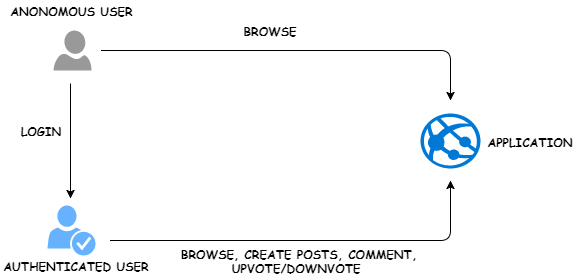
\includegraphics[width=19cm]{situation}
\caption{Current Situation Diagram}
\label{fig:env}
\end{figure}

\subsection {Business Data Model \& Data Dictionary}
\begin{figure}[H]
\centering
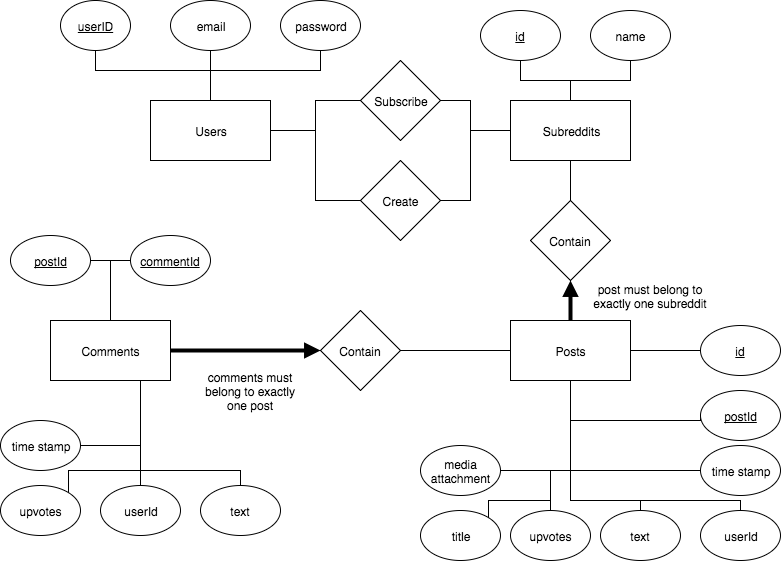
\includegraphics[width=16cm]{er}
\caption{ER Diagram}
\label{fig:ER}
\end{figure}

\begin{table}[H]
\caption{\bf Users schema}
\begin{tabularx}{\textwidth}{p{4cm}p{3cm}X}
\toprule {\bf Parameter} & {\bf Type} & {\bf Description}\\
\midrule
uid & String & Firebase assigned user id. \\
email & String & User's specified email address \\
password & String & User's specified user password. Password combined with email address allows users to access their account. \\
\bottomrule
\end{tabularx}
\end{table}

\begin{table}[H]
\caption{\bf Subreddits Schema}
\begin{tabularx}{\textwidth}{p{4cm}p{3cm}X}
\toprule {\bf Parameter} & {\bf Type} & {\bf Description}\\
\midrule
subredditId & String & Unique identifier of a subreddit.\\
name & String & Name of the subreddit. \\
\bottomrule
\end{tabularx}
\end{table}

\begin{table}[H]
\caption{\bf Posts Schema}
\begin{tabularx}{\textwidth}{p{4cm}p{2cm}X}
\toprule {\bf Parameter} & {\bf Type} & {\bf Description}\\
\midrule
postId & String & Unique identifier auto-assigned to post.\\
subredditId & String & id Referenced from Subreddit table that ties a post to a subreddit. \\
uid & String & userId referenced from Users table that ties a user to a post.\\
media\_attachment & String & URL or binary data (uploaded from device) \\
title & String & User specified title of the post \\
message & String & Text that belongs in the content of a post. \\
up-votes & Integer & Number modified as user's 'up-vote' a post or 'down-vote' a post. \\
time\_stamp & Number & UNIX timestamp of the  date at time of creation. \\
\bottomrule
\end{tabularx}
\end{table}

\begin{table}[H]
\caption{\bf Comments Schema}
\begin{tabularx}{\textwidth}{p{4cm}p{2cm}X}
\toprule {\bf Parameter} & {\bf Type} & {\bf Description}\\
\midrule
commentId & String & Unique identifier auto-assigned to comment. \\
postId & String & postId referenced from Posts table that ties a comment to a post.\\
uid & String & userId referenced from Users table that ties a user to a comment.\\
upvotes & Integer & Number modified as user's 'up-vote' a post or 'down-vote' a comment. \\
message & String & Content of the comment. \\
time\_stamp & Number & UNIX timestamp of the  date at time of creation. \\
\bottomrule
\end{tabularx}
\end{table}

\subsection {The Scope of the Product}
Below is the Use-Case Diagram for the User Interaction System.
\begin{figure}[H]
\centering
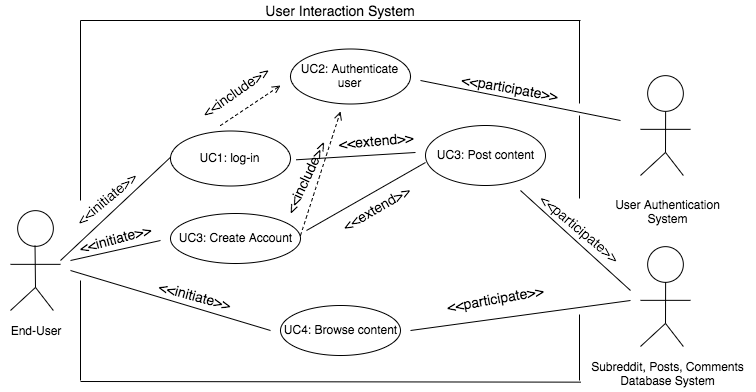
\includegraphics[width=16cm]{UseCase}
\caption{Use Case Diagram for the User Interaction System}
\label{fig:use-case}
\end{figure}

\subsection {Functional Requirements}

\begin{tcolorbox}
\textbf{Requirement Number: FR1}\\
\textbf{Description:} A user should be able to create a profile, log-in, log-out, and delete their profile.\\
\textbf{Rationale:} If the user cannot create a profile, they cannot create posts or contribute content.  Similarly, a user should have the right to permanently remove themselves from the application through deletion of their profile. \\
\textbf{Fit Criterion:} Able to create a user profile, verify through an email address, reset one's password, and delete application.
\end{tcolorbox}

\begin{tcolorbox}
\textbf{Requirement Number: FR2} \\
\textbf{Description:} A user who is logged in should be able to create a post within a subreddit. \\
\textbf{Rationale:} Any authenticated user should be able to post content. \\
\textbf{Fit Criterion:} Posts shall be created on multiple accounts.
\end{tcolorbox}

\begin{tcolorbox}
\textbf{Requirement Number: FR3} \\
\textbf{Description:} Any user should be able to browse content (not required to log-in). \\
\textbf{Rationale:} Users should not need to be authenticated when just browsing the application.\\
\textbf{Fit Criterion:} Both authenticated and anonymous users shall be able to browse through posts and comments in any subreddit.
\end{tcolorbox}

\begin{tcolorbox}
\textbf{Requirement Number: FR4} \\
\textbf{Description:} Users should be able to delete their posts and comments when logged on. \\
\textbf{Rationale:} Users should have control over the content and replies they submit. \\
\textbf{Fit Criterion:} Authenticated users shall have the ability to edit and delete their posts.
\end{tcolorbox}

\begin{tcolorbox}
\textbf{Requirement Number: FR5} \\
\textbf{Description:} A user should be able to create a comment in response to a post when logged on. \\
\textbf{Rationale:} Users should be able to discuss content posted. \\
\textbf{Fit Criterion:} Authenticated users shall be able to comment on posts.
\end{tcolorbox}

\begin{tcolorbox}
\textbf{Requirement Number: FR6} \\
\textbf{Description:} A user should be able to 'up-vote' or 'down-vote' posts and comments when logged on. \\
\textbf{Rationale:} Users should be able to have input on what they deem is interesting and be able to agree or disagree with other user's comments.  This will ensure the content on the application is user-curated. \\
\textbf{Fit Criterion:} Authenticated users shall be able to 'up-vote' and 'down-vote' posts or comments once.
\end{tcolorbox}

\begin{tcolorbox}
\textbf{Requirement Number: FR7} \\
\textbf{Description:} Posts can be sorted based on date posted and popularity.\\
\textbf{Rationale:} More popular or interesting posts(deemed by the community) should be shown to users with priority. \\
\textbf{Fit Criterion:} Posts with higher ratings shall be shown before lower rated posts.
\end{tcolorbox}

\begin{tcolorbox}
\textbf{Requirement Number: FR8} \\
\textbf{Description:} User profiles show karma points(accumulated from their posts or comments) \\
\textbf{Rationale:} Users submitting quality content or have comments which the community values should be awarded.\\
\textbf{Fit Criterion:} User profiles shall show their accumulated karma points from all of their posts and comments.
\end{tcolorbox}

\pagebreak
\section {Non-functional Requirements}

\subsection {Look and Feel Requirements}
\begin{tcolorbox}
\textbf{Requirement Number: NF1} \\
\textbf{Description:
 The GUI will be how the user interacts with the application.  The GUI should include a log-in/sign-up screen, content posted on the application and click-able buttons.  The buttons will allow the user to navigate the application as well as 'up-vote' and 'down-vote' content.  Content should be sorted based on popularity.  }  
\end{tcolorbox}

\subsection {Usability and Humanity Requirements}
\begin{tcolorbox}
\textbf{Requirement Number: NF2} \\
\textbf{Description:
The application will be able to be used by anyone that can use a keyboard and mouse, or a mobile device's keyboard and UI.}
\end{tcolorbox}

\subsection {Performance Requirements}
\subsubsection {Speed and Latency Requirements}
\begin{tcolorbox}
\textbf{Requirement Number: NF3} \\
\textbf{Description:
The application shall respond to user input to make subreddits, posts, and comments. The application data shall update with new subreddits, posts, comments as soon as the user opens the application, or manually refreshing the page.}
\end{tcolorbox}

\subsubsection{Reliability and Availability Requirements}
\begin{tcolorbox}
\textbf{Requirement Number: NF4} \\
\textbf{Description:
The application shall be available wherever there exists an internet connection and as long as the Firebase realtime database is under maximum load.}
\end{tcolorbox}

\subsubsection{Longevity Requirements}
\begin{tcolorbox}
\textbf{Requirement Number: NF5} \\
\textbf{Description:
The application will be relevant for the life of Angular 4 and Ionic 2/3, as well as Javascript functional browsers.}
\end{tcolorbox}
\subsection {Operational and Environmental Requirements}
\begin{tcolorbox}
\textbf{Requirement Number: NF6} \\
\textbf{Description:
The product is to be used anywhere where there exists an internet connection, and there exists a device that has access to an internet browser.}
\end{tcolorbox}
\subsection {Maintainability and Support Requirements}

\subsubsection{Maintenance Requirements}
\begin{tcolorbox}
\textbf{Requirement Number: NF7} \\
\textbf{Description:
The application will have minimal maintenance requirements. The domain name will have to be renewed yearly. Changes to visual styling may be made without affecting the functionality of the application itself.}
\end{tcolorbox}
\subsection {Security Requirements}
\begin{tcolorbox}
\textbf{Requirement Number: NF8} \\
\textbf{Description:
Each user profile is password protected. This protects others from logging into another user profile and posting/updated/deleting content that is not theirs. There is an option for user's to reset their password as well via a "Forgot your password?" button.}
\end{tcolorbox}

\subsection {Cultural Requirements}
Non-applicable.
\subsection {Legal Requirements}
\begin{tcolorbox}
\textbf{Requirement Number: NF9} \\
\textbf{Description: The application should adhere to all laws} 
\end{tcolorbox}
\pagebreak


\section {Project Issues}

\subsection {Open Issues}
Issues can be viewed on the reddit-clone \href{https://gitlab.cas.mcmaster.ca/trudeaua/reddit-clone/issues?scope=all&utf8=%E2%9C%93&state=all}{GitHub}. \\
\begin{enumerate}
\item \textbf{Back end database management; Closed as of October 1, 2017} \\
Authentication through Firebase has been completed but how the application manages data storing and data flow is still an issue. \\

\item \textbf{Posts can be created even when user is not logged in; Closed as of October 14, 2017}\\
When selecting "create a post" for the second time and the user does not exist or is not logged in, they will still be able to create a post. \\
Opened by: Kathryn Kodama \\
Closed by: Tommy Tran \\

\item \textbf{Browser issue; Closed as of October 21, 2017}
Application is not fully compatible with ES7 code (may want to switch to ES6).\\
Opened by: Alex Trudeau \\
Closed by: Alex Trudeau \\

\item \textbf{Mobile login not working on Android Google Chrome; Closed as of November 17, 2017}
When on mobile (Android) and trying to log in, when incorrect password or email entered cannot edit the entered fields. \\
Opened by: Kathryn Kodama \\
Closed by: Kathryn Kodama, Alex Trudeau - new version of Ionic seemed to fix this problem. \\

\item \textbf{Verification email inconsistencyl; Closed as of November 26, 2017} \\
Users should be able have resend a verification email in case the original for some reason is not received. \\
Opened by: Tommy Tran \\
Closed by: Kathryn Kodama \\

\item \textbf{Fresh clones of repository do not compile user metadata; Closed as of November 19, 2017} \\
When the Github repository is cloned an error occurs on the user metadata. \\
Opened by: Kathryn Kodama \\
Closed by: Tommy Tran, Alex Trudeau \\

\item \textbf{String .valueOf() does not work in some browsers; Closed as of November 25, 2017} \\
Opened by: Alex Trudeau \\
Closed by: Alex Trudeau \\

\item \textbf{User's subscribed subreddits not syncing with other devices; Closed as of November 25, 2017} \\
When a user unsubscribes from the mobile login it does not appear as unsubscribed on another device. \\
Opened by: Alex Trudeau \\
Closed by: Alex Trudeau \\

\end{enumerate}

\subsection {Off-the-Shelf Solutions}

\subsubsection{Ready-Made Products}
Since the application requires unique data management, it is not possible to purchase a solution.
\subsubsection{Products that can be copied}
The application is based off of the original Reddit so it is possible to observe the source code and try to mimic their solution.

\subsection {New Problems}
\subsubsection {Limitations in the Anticipated Implementation
Environment That May Inhibit the New Product}
Since the application is leveraging Firebase's free plan, if there are over 100 simultaneous connections or data transferred is over the allowed limit the application may not function correctly.
\subsubsection {Follow-Up Problems}
The application requires Firebase in order to function properly. If Firebase is shut down or offline there is nothing our developers can do about it.  Updates of Firebase can subsequently alter the compilation of the project and therefore the project must be updated accordingly.  

\subsection {Tasks}

\subsubsection{Project Planning}

\begin{table}[H]
\caption{\bf Project Planning }
\begin{tabularx}{\textwidth}{p{10cm}X}
\toprule {\bf Task} & {\bf Projected Finish Date}\\
\midrule
User authentication & October 14, 2017 \\
Subreddit, Post and Comment functionality & October 16, 2017 \\
User profiles and subreddit/post sorting & November 13, 2017 \\
Additional functionalities & November 27, 2017 \\
\bottomrule
\end{tabularx}
\end{table}

A more detailed breakdown of the project can be viewed via the Gantt chart on the reddit-clone \href{https://gitlab.cas.mcmaster.ca/trudeaua/reddit-clone.git}{GitHub}

\subsection {Risks}
As with any online open forum or discussion board, a health and safety risk associated with this project is cyber-bullying or online harassment. An additional health and safety risk associated with this application is strain on the eyes as it only operated through the screens of mobile devices or user's computers. There is also the case of copyright infringement or inappropriate content being posted. This will be up to the developers to prevent and curate while this application is in use.  The developers email will also be available for users to report specific cases of harassment or inappropriate use of the application. \\

Risks to be tested for the proof of concept are user security.  It is critical to test that the project will protect the email and passwords of its' users.  Additionally, the proof of concept should test for FR1, FR2, FR3, FR5, FR6.  The remaining functional requirements will be implemented and tested after the initial proof of concept.  The appropriate corresponding non-functional requirements will be tested as the functional requirements are tested. 

\subsection {Costs}
There will be no external costs involved in the implementation of the project because of the free hosting service provided by Google Firebase. However, if there are too many users or posts a premium Firebase plan may need to be purchased. 

\subsection {User Documentation and Training}
The project will include a "Help" page which will instruct users upon creation of a log-in on how to create subreddits, posts, and upvote content.  The GUI will be easy enough to navigate that documentation will not be needed for users in order to browse content.
\subsection {Waiting Room}
The following requirements are not to be included in the initial product release.
\begin{itemize}
\item Curating and moderating content including but not limited to appointing moderators.  This would require additional developers.
\item Additional functionality including new sorting methods for content.
\item Restriction of inappropriate content including an option for users to report other users, comments, posts, and subreddits.
\item A messaging systems for users to have one-on-one conversations.
\end{itemize}

For the first proof of concept the following functionalities were ready to roll out:  user authentication, creating posts, subreddits, comments and up-voting and down-voting content. \\

Beyond the proof of concept (for the final demo) the following functionalities were added: user profile, sorting posts and subreddits, reddit-clone themes and deleting comments and posts. 

\subsection {Ideas for Solutions}
Further insight on Firebase User authentication and security. 
Proper hierarchy, teamwork, and documentation of code with help to solve issues as they occur.

\end{document}
